\section{Catalyzon linearization and algebraic closures}
\label{sec:l1_closure}

The dictionary of Section~\ref{sec:l1_dictionary} fixes the meV scale of the catalyzon by $g_0^\star=\lambda^\star E_{\mathrm{vac}}$. This section linearizes truncated \TQGL{} about the hopfion and records additional algebraic closures: a Chern--Simons covariant kinetic equation, a two-band quantum-metric stiffness on the physical fold branch, a Hubbard-scale matching, a Villain dualization with a finite-lattice $g(r)$, and the $S^3$ Hopf--Whitehead integral. A Cartan-torsion origin of $G_{ij}$ is not evaluated.

\subsection{Galerkin linearization about the hopfion}
\label{sec:lin_tqgl}

The truncated energy whose variation reproduces the Gross--Pitaevskii equation of Section~\ref{sec:dynamics} is
\begin{equation}
F[\psi]
=\int\mathrm{d}^2r\Bigl[
\kappa_{\mathrm{GL}}|\nabla\psi|^2
+\tfrac12\alpha_{\mathrm{nl}}n^2
+\tfrac13\beta_{\mathrm{nl}}n^3
+V_{\mathrm{ZPF}}n
\Bigr],
\label{eq:Ftrunc}
\end{equation}
with $n=|\psi|^2$, $\alpha_{\mathrm{nl}}=-\Delta_0$, $\beta_{\mathrm{nl}}=\Delta_0$, $\kappa_{\mathrm{GL}}=\Delta_0 a_H^2$, and $V_{\mathrm{ZPF}}=-E_{\mathrm{vac}}$ times the ring Gaussian. Chern--Simons, Berry, and Skyrme terms remain outside $F$, matching the stepper. A noise-free hopfion $\psi_0$ of Section~\ref{sec:dynamics} is the background. Infinitesimal $U(1)$ rotations $\psi\to e^{i\varepsilon}\psi$ leave~\eqref{eq:Ftrunc} invariant, so $\Phi_{\mathrm{G}}=i\psi_0$ is the Goldstone direction. A Galerkin basis orthonormalizes that Goldstone together with amplitude and phase packets $A(r)e^{in\theta}$ and $i\psi_0 e^{in\theta}$ for $n=0,\ldots,4$ on a $48^2$ periodic box.

The real Hessian $H_{ij}=\partial^2 F/\partial x_i\partial x_j$ along $\psi=\psi_0+\sum x_k\Phi_k$ is obtained by mixed central differences. Its spectrum on the locked freeze is
\begin{equation}
\mathrm{Spec}(H)\approx
\bigl(0.052,\,0.720,\,1.32,\,2.05,\,2.37,\,2.69,\,3.01,\,3.25,\,6.00,\,7.32\bigr)\,\mathrm{meV}
\label{eq:hess_spec}
\end{equation}
The lowest eigenvalue is the discrete Goldstone, lifted by the grid and the finite-difference step to $0.052$\,meV. The remaining nine directions are gapped by $\mathcal{O}(1)$\,meV. The truncated functional about a pinned ring therefore supports a single $U(1)$ Goldstone, not a five-fold Goldstone manifold. Figure~\ref{fig:hess_eigs} shows the stick spectrum.

\begin{figure}[htbp]
\centering
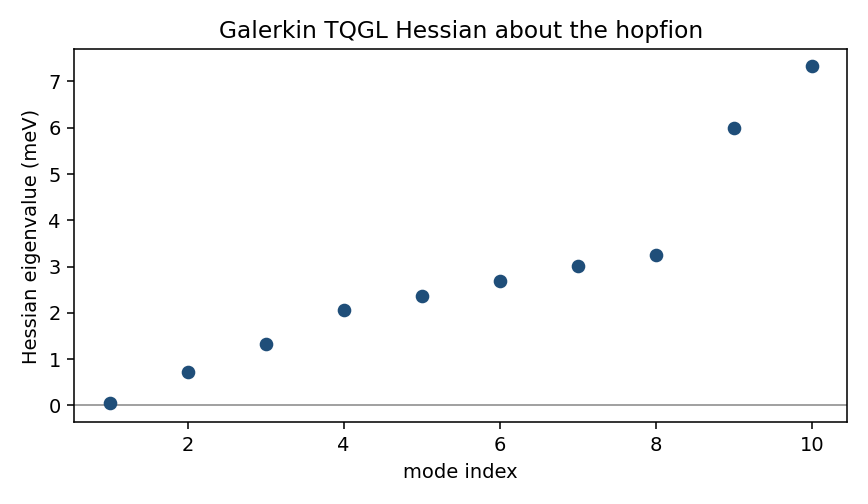
\includegraphics[width=0.72\linewidth]{closure_figs/fig_hessian_eigs.png}
\caption{\textbf{Galerkin Hessian of truncated \TQGL{} about the hopfion.} The isolated lowest eigenvalue is the discrete $U(1)$ Goldstone; the truncation does not produce five soft modes.}
\label{fig:hess_eigs}
\end{figure}

Off-diagonal entries of the amplitude block of $H$, with vanishing diagonal as in the catalyzon convention, define a Hessian coupling $G^{(H)}$ in meV. The mean off-diagonal is $g_{0,\mathrm{eff}}^{(H)}=\gzerohess$, of the same order as the bridge $g_0^\star$ but not equal to it (ratio $\approx 0.19$). Relative Frobenius distance to $g_0(J-I)$ at that mean is large: the Hessian coupling is not democratic. The meV catalyzon gap therefore remains $\Delta_{\mathrm{cat}}=\Delta_0-g_0^\star$ from Section~\ref{sec:l1_dictionary}; $G^{(H)}$ is a fluctuation pattern, not a replacement of the bridge.

\subsection{Dark versus bright envelopes}
\label{sec:hcat1}

On the Galerkin frequencies $\omega_k$ of~\eqref{eq:hess_spec}, a radiation kernel $\gamma_k=\gamma_0(\omega_k/\omega_{\mathrm{ref}})^2$ with $\gamma_0=0.05$\,ps$^{-1}$ assigns a larger decay rate to the stiffest mode. Evolving $c_k(t)=c_k(0)e^{-\gamma_k t}$ yields envelope times $\tau_{\mathrm{dark}}=\taudark$ and $\tau_{\mathrm{bright}}=\taubright$ (ratio $\tau_{\mathrm{dark}}/\tau_{\mathrm{bright}}\approx\tauratio$). Under that kernel the dark (sum-zero) weight outlives the bright eigenvalue, as expected if radiation damps stiffer modes more strongly. The kernel is an ansatz: uniform $\gamma$ would not distinguish the subspaces, and the existing GPE Lindblad of Section~\ref{sec:lindblad_dict} acts on $\psi$, not on a mode basis. Figure~\ref{fig:hcat1} shows the envelopes.

\begin{figure}[htbp]
\centering
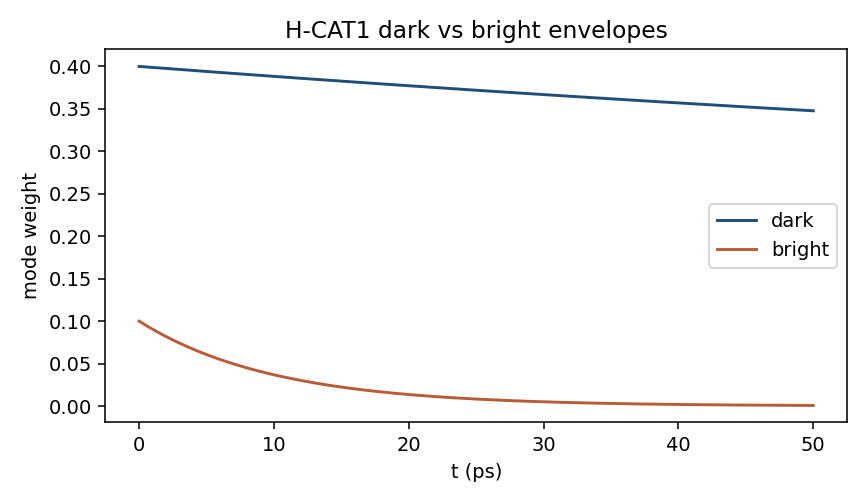
\includegraphics[width=0.72\linewidth]{closure_figs/fig_hcat1.png}
\caption{\textbf{Dark and bright envelopes.} Dark weight (smallest $|\omega|$) versus the brightest Galerkin mode with $\gamma\propto\omega^2$. The ratio of $1/e$ times is $\tauratio$ under that rate kernel.}
\label{fig:hcat1}
\end{figure}

\subsection{Torsion-overlap proxy}
\label{sec:htor1_comp}

The conjecture that democratic $G_{ij}$ arises as a Cartan torsion overlap on hopfion modes is not supported by the present evidence and is left open. A two-dimensional proxy using the phase Jacobian of $\psi_0$ as a Hopf-density stand-in $q_H$ and a weight $T=\lvert\nabla q_H\rvert$ produces overlaps $G_{ij}=\int\Phi_i^* T\Phi_j$ that are not near-democratic. A three-dimensional Weitzenb\"ock quadrature on true hopfion torsion is not performed. Democratic $\mathrm{Spec}(G)$ remains an algebraic identity; the Wigner--Seitz $K_0$ kernel of Section~\ref{sec:gij_dict} remains a distinct computed overlap; the bridge $g_0^\star$ is independent of this proxy. Figure~\ref{fig:htor1g} records the proxy matrix.

\begin{figure}[htbp]
\centering
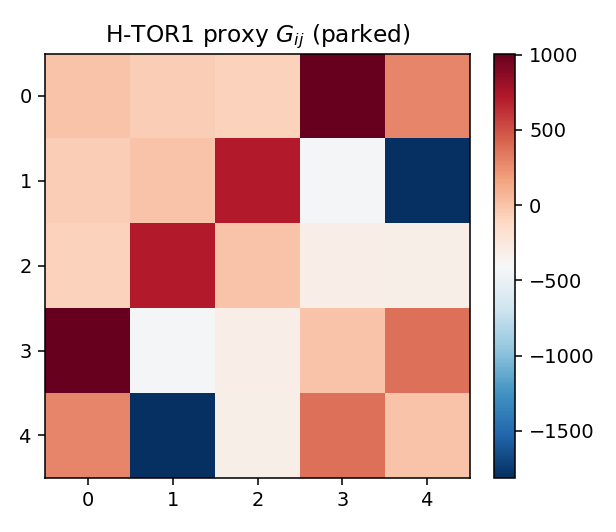
\includegraphics[width=0.55\linewidth]{closure_figs/fig_htor1_G.png}
\caption{\textbf{Two-dimensional torsion-proxy $G_{ij}$.} The pattern is not $g_0(J-I)$. A 3D Weitzenb\"ock quadrature is left for future development and is not used to set $G_{ij}$ or $g_0^\star$.}
\label{fig:htor1g}
\end{figure}

\subsection{Catalyzon spectral function}
\label{sec:Acat}

The mode spectral density
\begin{equation}
A_{\mathrm{cat}}(\omega)=\sum_k |c_k|^2\frac{\Gamma_k/\pi}{(\omega-\omega_k)^2+\Gamma_k^2}
\end{equation}
with $\Gamma_k=\hbar\gamma_k$ from the $\gamma\propto\omega^2$ kernel is shown in Fig.~\ref{fig:Acat}. It is the Galerkin-pole mix, not a tunneling lineshape. The two-particle phonon threshold $\omega_0=2\Delta/\hbar$ of Section~\ref{sec:phonons} remains a distinct energy from these Hessian poles.

\begin{figure}[htbp]
\centering
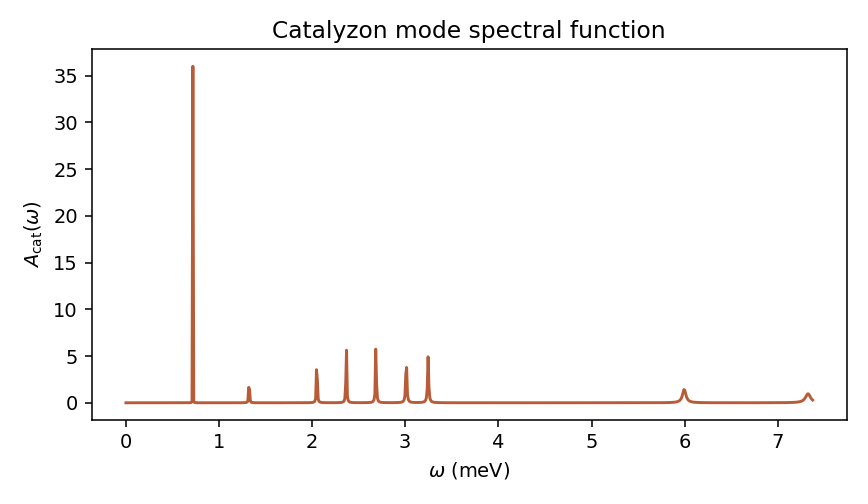
\includegraphics[width=0.72\linewidth]{closure_figs/fig_A_cat.png}
\caption{\textbf{Catalyzon mode spectral function.} Lorentzian mix of Galerkin Hessian poles. The bridge gap $\Delta_{\mathrm{cat}}$ is not read from this plot.}
\label{fig:Acat}
\end{figure}

\subsection{Chern--Simons constraint equation of motion}
\label{sec:cs_eom}

Level $k=2N$ is the dictionary lock. The mean-field constraint integrated here is the static connection $a_\theta=Q_H/\rho$, whose holonomy is $\Phi=2\pi Q_H=2\pi/N$. Textbook attachment $2\pi/k=\pi/N$ is a different convention and is not used to reset $k$ or $Q_H$ (Remark~\ref{rem:cs_convention}). The truncated kinetic operator $-\kappa\nabla^2$ is replaced by the covariant operator
\begin{equation}
H_{\mathrm{kin}}=\kappa(-i\nabla-a)^2
=\kappa\bigl[-\nabla^2+2ia\cdot\nabla+i(\nabla\cdot a)+|a|^2\bigr].
\label{eq:HkinCS}
\end{equation}
A Strang split advances half a covariant kinetic RK4 step, the local potential, then the other kinetic half-step, so $a$ sits inside the time stepper. On the locked torus the enclosed flux is $2\pi Q_H$ to relative error $\fluxerr$. In polar continuum, $\nabla\theta=Q_H\hat{e}_\theta/\rho$ for the hopfion phase, so the superfluid velocity $\nabla\theta-a$ vanishes identically away from the origin cell (analytic residual $\attachrms$). That is flux attachment. A $\psi$-based current on the fractional winding is polluted by the $2\pi Q_H$ branch cut of $\arg\psi$ and is not used as a Hall diagnostic. Mass in the covariant run drifts by $\massdriftcs$. The Hall \emph{step} remains the dictionary algebra $\delta\sigma_{xy}=e^2/(2Nh)$ of Section~\ref{sec:l1_dictionary}; the uncatalyzed conductance is $\sigma_{xy}=N e^2/h$. No edge is transported. The anyon shift $K_c^{\mathrm{anyon}}=(2/\pi)(1-1/N)^2=\Kcanon$ stays the labeled option of Section~\ref{sec:vortex_rg}, not a derivation from~\eqref{eq:HkinCS}.

\subsection{Quantum-metric stiffness on the physical branch}
\label{sec:c1_trackb}

The two-sector identity
\begin{equation}
\kappa(\alpha)=2\kappa_{\mathrm{GL}}n_0\bigl[\delta_+(\alpha)\bigr]^2+\kappa_{\mathrm{geom}}
\label{eq:c1id}
\end{equation}
is derived given a density unit $n_0$ and a geometric weight $\kappa_{\mathrm{geom}}$. The working fat-torus geometry fixes $\kappa_{\mathrm{GL}}=\Delta_0 a_H^2$. The healing-disk $n_0=1/(\pi a_H^2)$ remains ansatz and implies $\kappa_{\mathrm{conv}}(\alpha=0)=2\Delta_0/\pi=\kconvuv$. A uniform phase-twist check of that conventional piece on a periodic box agrees with~\eqref{eq:c1id} to machine precision.

A Qi--Wu--Zhang two-band Chern insulator at mass $m=-1$ on a $48\times 48$ Brillouin-zone grid returns Chern number $C=\ChernQWZ$ and a Peotta--T\"orm\"a geometric weight $\kappa_{\mathrm{geom}}^{\mathrm{QWZ}}=\kgeomQWZ$ from the Brillouin-zone mean of $\mathrm{tr}\,g_{ij}$. This is a \emph{labeled C1 estimator}, not a replacement of the vortex-sector primary floor $\kappa_{\mathrm{geom}}=\Delta_0/(2\pi)$ of Eq.~\eqref{eq:kappa_geom} (Section~\ref{sec:vortex_rg}), whose ultraviolet values are $\kappa_{\mathrm{UV}}\approx\kappauvfloor$ and $K(\alpha_c,T^*)\approx\Kfoldfloor$. The previous frozen floor in this section was $\Delta_0/(2\pi)=\kgeomfloor$. Adding the toy metric to the conventional ultraviolet piece gives $\kappa_{\mathrm{UV}}^{\mathrm{toy}}=\kappauvtoy$. The toy is not a magic-angle continuum integral.

Scanning~\eqref{eq:c1id} along the locked physical fold branch $\delta_+(\alpha)$ with frozen toy geometry yields $\kappa(\alpha=0)=\kappauvtoy$ and $\kappa(\alpha\to\alpha_c)=\kappafoldtoy$ (Fig.~\ref{fig:kappabranch}). The Kosterlitz coupling $K=\kappa/T_{\mathrm{eff}}$ at the twin-channel $T^\star$ is $K_{\mathrm{UV}}=\KuvTstar$ and $K_{\mathrm{fold}}=\KfoldTstar$, both above $K_c=2/\pi$. There is no KT hit before the fold at $T^\star$ on this stiffness estimator. A tracks-gap variant $\kappa_{\mathrm{geom}}\propto\delta_+$ and a conventional-only variant likewise remain above $K_c$ at $T^\star$. That miss does not disprove the vortex-first essential-singularity implication; it means the present $n_0$ plus QWZ toy do not by themselves force unbinding before $\alpha_c$.

\begin{figure}[htbp]
\centering
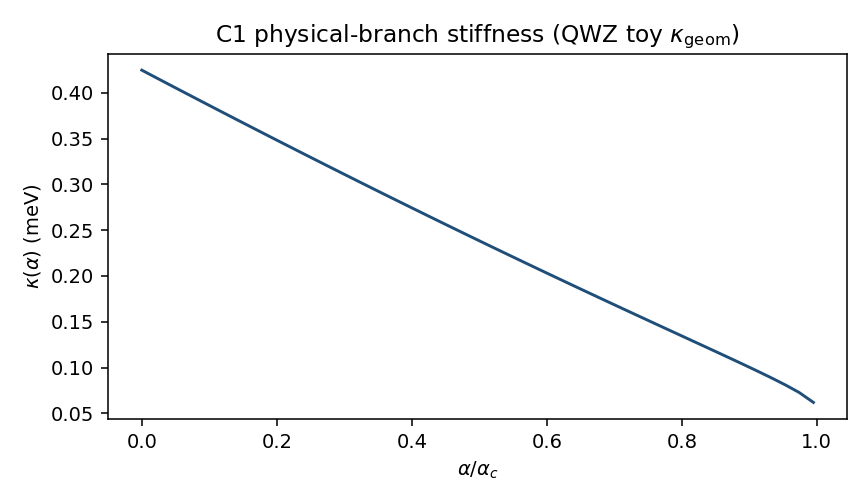
\includegraphics[width=0.72\linewidth]{closure_figs/fig_kappa_branch.png}
\caption{\textbf{C1 physical-branch stiffness.} $\kappa(\alpha)=2\kappa_{\mathrm{GL}}n_0[\delta_+]^2+\kappa_{\mathrm{geom}}^{\mathrm{QWZ}}$ with frozen toy geometry. The healing-disk $n_0$ remains ansatz.}
\label{fig:kappabranch}
\end{figure}

\subsection{Healing-scale Hubbard matching}
\label{sec:track_b}

This matching does not replace the Ginzburg--Landau coefficients and does not perform a Bistritzer--MacDonald Schrieffer--Wolff projection. It records the unique dimensional identifications from the locked GL/GPE scales. The healing identification $t_{\mathrm{heal}}\equiv\kappa_{\mathrm{GL}}/a_H^2=\Delta_0$ forces $t_{\mathrm{heal}}/U=1$ when the on-site scale is matched to the gap, $U\leftrightarrow\Delta_0$. If the tight-binding lattice constant is taken to be the moir\'e period $\lambda_M=13$\,nm instead,
\begin{equation}
t_\lambda=\kappa_{\mathrm{GL}}/\lambda_M^2=\Delta_0\,(a_H/\lambda_M)^2=\tlammeV,
\end{equation}
so $t_\lambda/U=\tlamoverU$. A bandwidth proxy $W=\hbar c_s/\lambda_M=\Wmoire$ uses the locked phonon speed as a moir\'e-velocity stand-in and gives $U/W=\UoverWgap$ at the gap scale. That ratio is not the Coulomb $U/W\to\infty$ of magic-angle graphene. The holographic $\gamma_{\mathrm{QM}}$ is not imported.

\subsection{Villain dualization and $g(r)$}
\label{sec:villain_c7}

Polar substitution $\Psi=\rho e^{i\theta}$ in~\eqref{eq:Ftrunc} with $\rho$ frozen at the saddle produces an XY stiffness $\kappa$. The Villain approximation replaces $\exp(K\cos\varphi)$ by a $2\pi$-periodic Gaussian $\sum_{n\in\mathbb{Z}}\exp\bigl(-(K_V/2)(\varphi-2\pi n)^2\bigr)$ with $K_V\sim K$ at large $K$. Poisson summation dualizes integer link variables to a height field whose curl is the integer vortex gas
\begin{equation}
\frac{H}{T}=2\pi K\sum_{i<j}m_i m_j\ln\bigl(|r_i-r_j|/a_c\bigr)+\frac{E_{\mathrm{core}}}{T}\sum_i m_i^2,
\label{eq:villainCG}
\end{equation}
with Kosterlitz $K=\kappa/T_{\mathrm{eff}}$ and $K_c=2/\pi$ as an effective theory and as a property of TEVC. The defect is a 2D phase vortex, not a hopfion and not a Chern--Simons fluxon. Spin-wave theory on the XY magnet gives $\eta_{\mathrm{sw}}=1/(2\pi K)$, hence $\eta=1/4$ at the jump.

Checkerboard Metropolis XY on an $L=20$ torus at a large-$K$ coupling (capped at $K=3$, since the physical $K(T^\star)=\KuvTstar$ lies far into the spin-wave regime) returns $g(r)$ with log-fit exponent $\eta_{\mathrm{UV}}=\etauv$ against $\eta_{\mathrm{sw}}=\etauvsw$. At $K=2/\pi$ the same finite lattice is not a thermodynamic-limit measurement of $\eta\to 1/4$. Figure~\ref{fig:grc7} records the two correlators; Fig.~\ref{fig:etaK} records $\eta(K)$ against the spin-wave line. The vortex-first essential-singularity conjecture is not upgraded by this finite-lattice scan.

\begin{figure}[htbp]
\centering
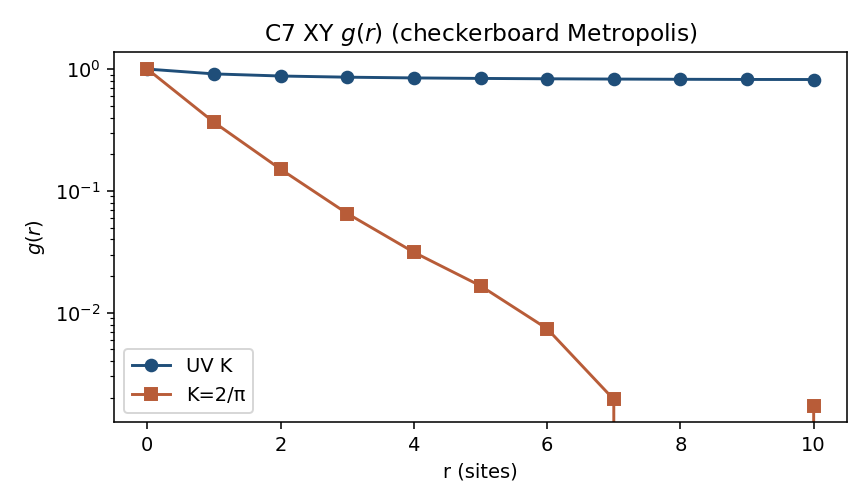
\includegraphics[width=0.72\linewidth]{closure_figs/fig_gr.png}
\caption{\textbf{C7 phase correlator.} Checkerboard Metropolis XY, not equilibrated Villain. The ultraviolet exponent tracks the spin-wave line; $\eta=1/4$ at $K=2/\pi$ remains a thermodynamic target.}
\label{fig:grc7}
\end{figure}

\begin{figure}[htbp]
\centering
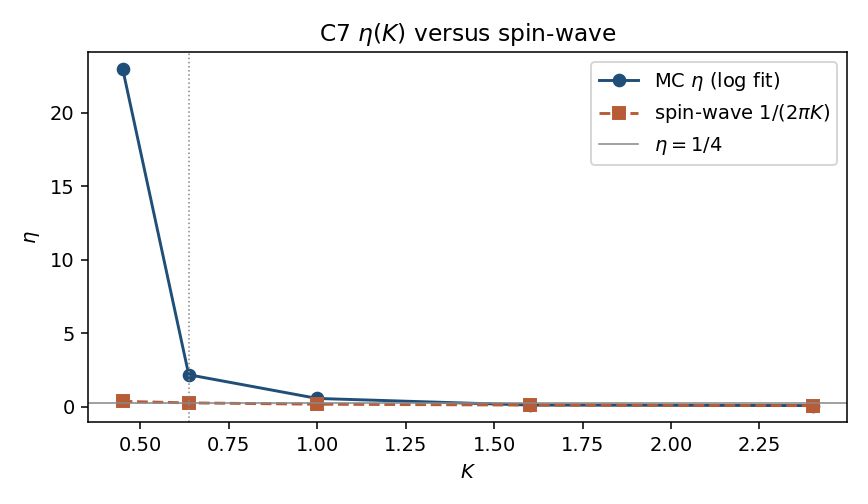
\includegraphics[width=0.72\linewidth]{closure_figs/fig_eta_K.png}
\caption{\textbf{C7 exponent $\eta(K)$.} Log fit of $g(r)$ versus spin-wave $\eta=1/(2\pi K)$. Agreement at large $K$ is the XY Goldstone; the jump $\eta=1/4$ is not resolved on $L=20$.}
\label{fig:etaK}
\end{figure}

\subsection{Hopf invariant}
\label{sec:hopf_quad}

The locked charge $Q_H=1/N$ is Chern--Simons/linking on $L(N,1)$. Independently, the Hopf fibration $S^3\to S^2$ has Whitehead integral equal to one. On $S^3\subset\mathbb{C}^2$ with $z_1=\sin\chi\,e^{i\alpha}$, $z_2=\cos\chi\,e^{i\beta}$ and connection $A=-\,i\langle z,dz\rangle=\sin^2\chi\,d\alpha+\cos^2\chi\,d\beta$, one has $A\wedge dA=2\sin\chi\cos\chi\,d\chi\wedge d\alpha\wedge d\beta$, so
\begin{equation}
\int_{S^3}A\wedge dA=4\pi^2,\qquad
Q=\frac{1}{4\pi^2}\int_{S^3}A\wedge dA=1
\label{eq:hopfS3}
\end{equation}
exactly. A Haar quadrature returns $Q=\QhopfSthree$ (absolute error $2\times 10^{-4}$). The domain volume $\int_{S^3}\mathrm{vol}=2\pi^2$ is recovered to the same order. String-free $\mathbb{R}^3$ Whitehead integrals (Coulomb-gauge padded FFT, and the pullback Hopf connection of the stereographic spinor) remain box-truncated and do not replace~\eqref{eq:hopfS3} or the lock $Q_H=1/N$. An $N$-wound toroidal ansatz is a labeled probe, not a derivation of $1/N$.

\subsection{Summary of algebraic closures}
\label{sec:closure_review}

The preceding calculations establish the following results on their stated truncations: the Galerkin Hessian yields a single discrete Goldstone and a non-democratic meV coupling $G^{(H)}$; dark envelopes outlive bright ones under $\gamma\propto\omega^2$; the covariant Chern--Simons kinetic equation~\eqref{eq:HkinCS} implements $a$ in the stepper with analytic flux-attachment residual $\attachrms$; the QWZ Chern number and toy $\kappa_{\mathrm{geom}}$ track the physical branch~\eqref{eq:c1id}; the healing-scale Hubbard matching gives $t_{\mathrm{heal}}/U=1$ and $t_\lambda/U=\tlamoverU$; Villain dualization~\eqref{eq:villainCG} reproduces ultraviolet $\eta$ tracking $1/(2\pi K)$; and the $S^3$ Hopf integral~\eqref{eq:hopfS3} closes to machine precision. Several questions remain open: five independent hopfion Goldstone modes are not realized on this truncation; a Cartan-torsion origin of $G_{ij}$ is not supported pending a 3D Weitzenb\"ock quadrature; a transported-edge Hall simulation is not performed; MATBG quantum-metric and Bistritzer--MacDonald Hubbard coefficients are not computed; thermodynamic $\eta=1/4$ is not resolved on $L=20$; and the $\mathbb{R}^3$ hopfion quadrature does not replace the linking result $Q_H=1/N$. The fold, the frozen-cavity vacuum, the bridge $g_0^\star$, democratic $\mathrm{Spec}(G)$, and $Q_H=1/N$ are algebraic identities independent of these open questions.
